\documentclass[12pt]{article}
\usepackage{graphicx}
\usepackage {color}
\usepackage{pdfpages}
\usepackage{float}
\usepackage{changebar}
\usepackage{enumitem,amssymb}
\renewcommand{\familydefault}{\sfdefault}
\usepackage[margin=1.2in]{geometry}
\usepackage{graphicx}
\usepackage{wrapfig}
\usepackage[super]{cite}
\usepackage{subcaption}
\usepackage[table]{xcolor}
\usepackage{amsmath}
\usepackage[sort, numbers]{natbib}
\usepackage{multirow}
\usepackage{tabularx}
\usepackage{siunitx}
\usepackage{matlab-prettifier}
%%%%%%%%%%%%Defining the margins %%%%%%%%%%%%%%%%%%%%%
\textheight 9.in
\textwidth 6.5in
\topmargin -.5in
\oddsidemargin 0in
\setlength{\parskip}{\smallskipamount}

%%%%%%%%%%%%%%Specific Commands %%%%%%%%%%%%%%%%%%
\newcommand{\eg}{{\em e.g.,}}
\newcommand{\ie}{{\em i.e.,}}
\newcommand{\etc}{{\em etc.,}}
\newcommand{\etal}{{\em et al.}}
\newcommand{\degrees}{{$^{\circ}$}}
\newcommand{\fig}[1]{\textbf{Figure #1}}

%%%%%%%%%%%%%%%%%%%%%%%%%%%% Setting to control figure placement
% These determine the rules used to place floating objects like figures 
% They are only guides, but read the manual to see the effect of each.
\renewcommand{\topfraction}{.9}
\renewcommand{\bottomfraction}{.9}
\renewcommand{\textfraction}{.1}
\renewcommand{\familydefault}{\sfdefault} %setting the san serif font

%%%%%%%%%%%%%%%%%%%%%%%% Line spacing
% Use the following command for ``double'' spacing
%\setlength{\baselineskip}{1.2\baselineskip}
% and this one for an acceptable NIH spacing of 6lpi based on 11pt
%\setlength{\baselineskip}{.9\baselineskip}
% The baselineskip does not appear to work when we include a maketitle
% command in the main file.  Something there must set the line spacing
% If we use this next command, then things seem to work.
\renewcommand{\baselinestretch}{.9}

\setcounter{secnumdepth}{0} %make no numbers but have a table of contents


\begin{document}

\title{HW 3: Medical Imaging Systems}
\author{Jake Bergquist, u6010393 }
\maketitle

\section{Q1}
\noindent\textbf{a: }
For question 1 I have re-drawn the sequence on the attached pages as can be seen in Drawing 1.  The colors used correspond to the traversal of the K space in Drawing 2. On Drawing 2 a solid line designates a sampling and a dotted line signifies a traversal of the K space without sampling. The $G_X$ axis is shown in red and the $G_Y$ axis is shown in blue. The numbers labeling the traversals of the K space on Drawing 2 correspond to the different pulses in the sequence depicted in Drawing 1. In each case all of the $G_X$ pulses are assumed to be equal (having equal area under the curve) except for the first $G_X$ pulse which is assumed to have a an area under the curve that is half that of the subsequent ones. All of the $G_Y$ pulses are assumed to have equal magnitude of area under the curve (some being negative). All traversals of the K space are thus given in a unit length. Following the trajectory from the origin first there is a dephasing pulse on $G_X$ (1) that moves us to a position in the positive direction on the $G_X$ axis of the K space to (1,0). Then there is a 180 pulse (2) that causes a traversal to a place on the negative $G_X$ axis to (-1,0). Next there is a $G_y$ pulse (3) that moves us to (-1.1) in the K space, followed by the first acquisition pulse (4) which acquires samples as we move from (-1,1) to (1,1). Next there is an inversion (5) that moves us to (-1,-1) followed by a negative $G_Y$ pulse (6) that moves us to (-1,-2). Then another acquisition(7) as we move to (-1,-2) to (1,-2). Then an inversion (8) to (-1,2). Then a positive $G_Y$ (9) to move to (-1,3). Then an acquisition (10) as we move to (1,3). Then an inversion (11) to (-1,-3). Then a negative $G_Y$ (12) to move to (-1,-4). Then the final acquisition as we move to (1,-4).

\noindent\textbf{b: } Drawing 3 shows the modifications to the sequence and the subsequent K space trajectories. In order to sample only in the positive $G_y$ area of the K space with lines like we did in part A first we allow the same $G_x$ positioning pulse (1) to move to a positive X position(1,0). Next we allow the 180 degree RF pulse to put us a (-1,0), followed by the first acquisition as we move to (1,0) again. From here there are many choices on how to use the $G_y$ to get us to a starting position where we can take another sample, prefereably at (-1,1). I chose to have a negative $G_y$ pulse (4) move us to (1,-1), then the subsequent inversion (5) will move us to the desired (-1,1) where we can take the next acquisition as we move to (1,1) using a $G_x$ pulse (6). Next we need another negative $G_y$ pulse (7) with the same area under the curve as pulse 4 to move us to (1,0) before the 180 RF (8) moves us to (-1,0). Now we need a $G_y$ pulse (9) with twice the area under the curve as 4 or 7, and this time it is a positive pulse to move us to (-1,2). Following this is a $G_x$ acquisition (10) that takes us to (1,2), folowed by a negative $G_y$ pulse (11) with twice the area under the curve as 4 or 7, taking us to (1,0), then a 180 flip (12) to get to (-1,0). Next we have a positive $G_y$ (13) with three times the area under the curve as 4 or 7 to get to (-1,3) and a final acquisition $G_x$ pulse (14) to get to (1,3). In contrast with the pervious sequence which was able to sample the K space at successivly greater distances from the origin, while mantaining the same amount of energy input to the gradients for each cycle, this sequence requires increasing energy to be provided to the $G_y$ coil in order to perform the proper K space positioning, making this sequence more difficult and costly to perform from an energy expenditure stance. Also it becomes mroe and more difficult to increase the area under the curve for the $G_y$ pulses without increasing the time of the pulse, which would hamper the speed of the sequence.

\section{Q2}
\noindent\textbf{a: }
Looking at sequence a it was clear that I would achieve this sort of pattern using sin and cos waveforms of the two gradients.  However simply using a sin for one gradient and a cos for the other would result in a circular trajectory in the K space when the two were integrated and used to plot the K space trajectory. Thsu there needed to be a term that started at zero and constantly increased as time went on such that the amplitudes of the sin and cos functions would increase result in spirals. The easiest way to do this was to multiply the function defining the waveform by time. My initial sketch for what this shouldlook like in the pulse sequence is shown in Drawing  4. Note that after excitation the acquistion is constant as the $G_x$ and $G_y$ change in the linearly increasing sinusiodal waveform.

The second sequence was not as easily drawn out with simple trig function. It shows a repetitive sequence of alternating directions of $G_x$ pulses interpsaced with negative $G_y$ pulses to advance the sampling through the K space. There is first an initial positiing pulse on both gradients to get tot he starting position. These Sequences are depicted in Drawing 5.

\noindent\textbf{b: }
The matlab code below was used to generate k-space sampling matching those presented. I had to change around the sina nd cos functions for the spiral plot a few times to make sure it started in the proper position and went in the proper direction. The resulting K space sampling is shown in Figure~

\begin{lstlisting}[style=Matlab-editor]
%
\end{lstlisting}

\section{Q3}



\end{document}



\begin{figure}[H]
	\centering
	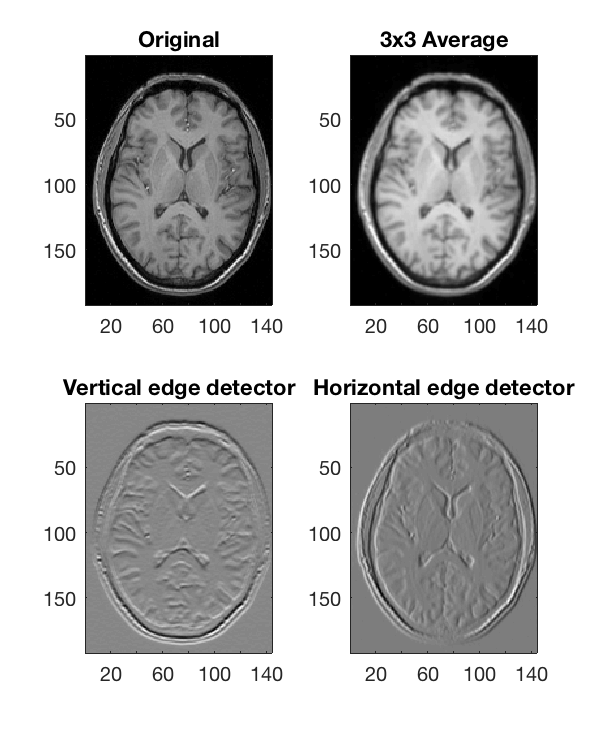
\includegraphics[width=\textwidth]{Figures/convs.png}
	\caption{}
	\label{Fig:conv}
\end{figure}






